\newpage
\hypertarget{treeToModel vis}{}
\subsection{The visual transformation rules}
\visHeader

A quick note before you start -- we assume a basic understanding of TGGs and the different ways of using EA productively to create rules. If you find this
section challenging, we recommend first working through Part IV to cover TGG fundamentals.

\begin{itemize}

\subsubsection{FolderToLibraryRule} % ---------------------------------

\item[$\blacktriangleright$] Return to EA and expand code adapter's \texttt{<<Rules Package>>}, then open the \texttt{Rules} diagram. Create a new rule
named \texttt{FolderToLibraryRule} and double-click the new diagram element to open its diagram. Complete the rule as depicted in
Fig.~\ref{ea:FolderIntoLibrary_Complete}. We established the \texttt{FolderToLibrary} correspondence type when creating the TGG schema in Section 1.

\vspace{0.5cm}

\begin{figure}[htbp]
\begin{center}
  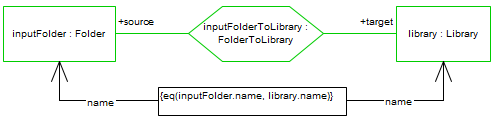
\includegraphics[width=\textwidth]{ea_FolderToLibraryRule}
  \caption{\texttt{FolderToLibraryRule}}
  \label{ea:FolderIntoLibrary_Complete}
\end{center}
\end{figure}

\item[$\blacktriangleright$] This is a simple rule that creates and connects equivalent \texttt{Folder} and \texttt{Library} instances and we're able to use
this entire rule as context for the next rule, which will handle the creation of shelves. Select \texttt{inputFolder},
\texttt{in\-put\-Fol\-der\-To\-Lib\-rary,} and \texttt{library}, then use the eMoflon control panel to \texttt{derive} a new rule (Fig.~\ref{ea:controlPanel}).
Name this \texttt{ForAllShelfRule}.

\vspace{0.5cm}

\begin{figure}[htbp]
\begin{center}
  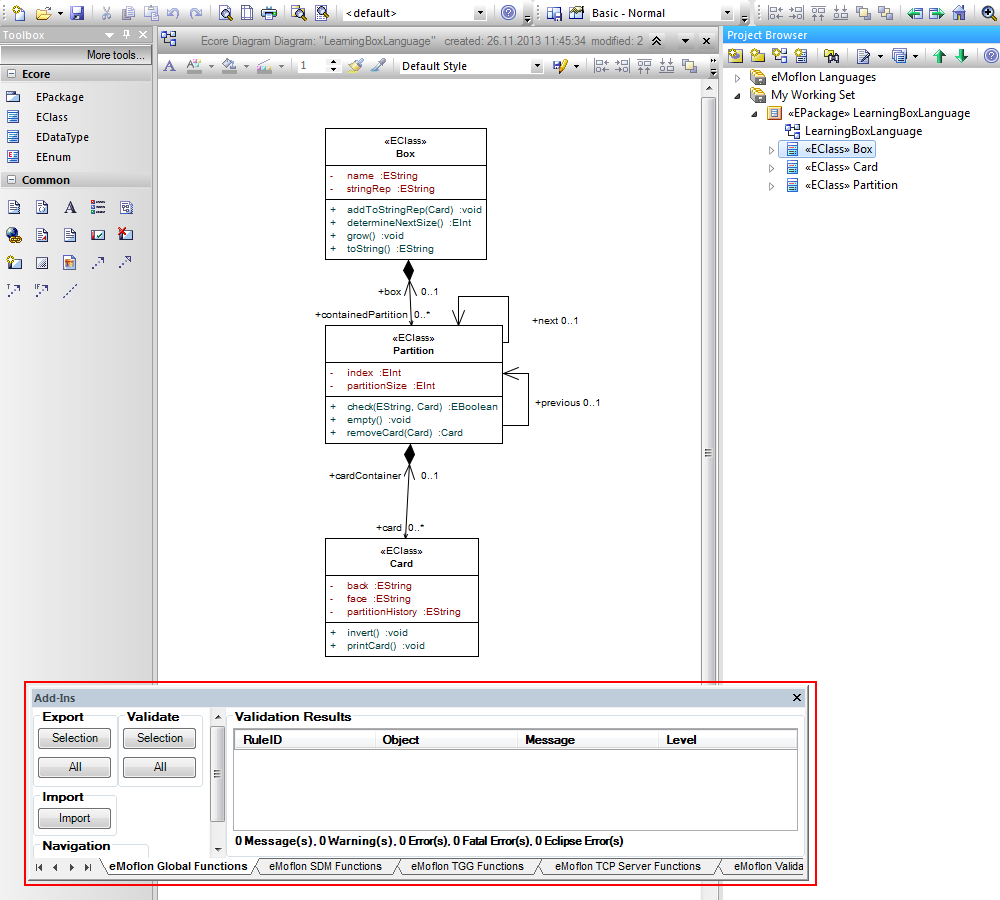
\includegraphics[width=\textwidth]{ea_controlPanel}
  \caption{Deriving a new rule with eMoflon's control panel}
  \label{ea:controlPanel}
\end{center}
\end{figure}

\newpage

\subsubsection{ForAllShelfRule} % ---------------------------------

\item[$\blacktriangleright$] The derivation procedure will open a new diagram with context elements from the first rule. This rule is similar to
\texttt{FolderToLibraryRule}, except that it will connect new (green) elements to existing (black) containers. Complete it as depicted in
Fig.~\ref{ea:ForAllShelves_Complete}.

\item[$\blacktriangleright$] You'll need to create a new \texttt{FolderToShelf} correspondence type in either the schema (as we did in the beginning), or
on-the-fly by selecting \texttt{Create New Correspondence Type} in the quick-link dialogue (Fig.~\ref{ea:corrOnTheFly}).

\begin{figure}[htbp]
\begin{center}
  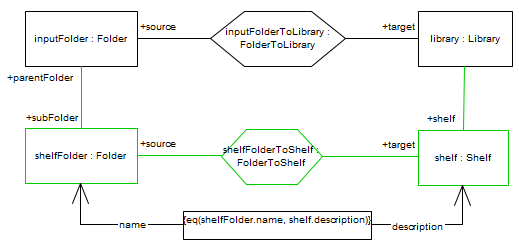
\includegraphics[width=0.9\textwidth]{ea_ForAllShelfRule}
  \caption{\texttt{ForAllShelfRule}}
  \label{ea:ForAllShelves_Complete}
\end{center}
\end{figure}

\begin{figure}[htbp]
\begin{center}
  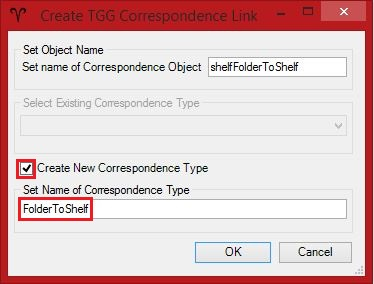
\includegraphics[width=0.6\textwidth]{ea_createNewLink}
  \caption{Creating a \texttt{FolderToShelf} correspondence type on-the-fly}
  \label{ea:corrOnTheFly}
\end{center}
\end{figure}

\subsubsection{NodeToDictionaryRule} % ---------------------------------

\item[$\blacktriangleright$] We are now ready to handle the dictionary \texttt{File} elements. Analogously to how you began the previous rule, select
\texttt{shelfFolder}, \texttt{FolderToShelf}, and \texttt{shelf}, and derive \texttt{NodeToDictionaryRule} with this context.

\item[$\blacktriangleright$] Complete it as depicted in Fig.~\ref{ea:NodeToDictionary_Complete}. As you can see, this rule creates a 
\texttt{dictionaryNode} and and its equivalent \texttt{dictionary}, and handles the first node in the tree structure. Nearly every
element is used to correctly set the \texttt{dictionary} and \texttt{dictionaryFile} names in two constraints.

\begin{figure}[htbp]
  \hspace{-0.7cm}
  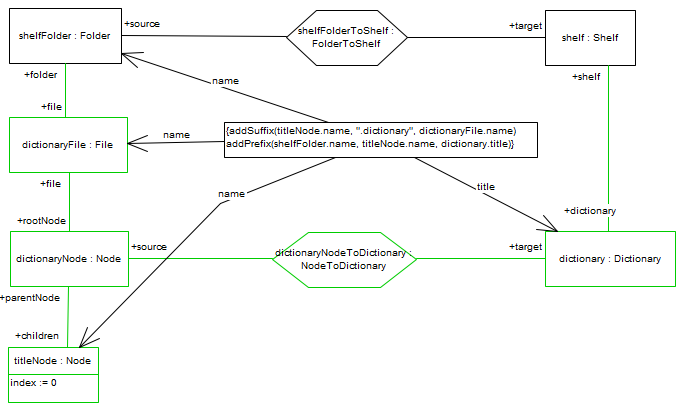
\includegraphics[width=1.2\textwidth]{ea_NodeToDictionaryRule}
  \caption{\texttt{NodeToDictionaryRule}}
  \label{ea:NodeToDictionary_Complete}
\end{figure}

\item[$\blacktriangleright$] Please note that the attribute constraint in \texttt{titleNode} is required in order to ensure that the node
with the title information is always the first child in the tree (index = 0). 

\item[$\blacktriangleright$] Note that we could have also included another \texttt{node} here to handle the author, then a third, fourth, or even tenth
\texttt{node} for the entries, but that would mean the pattern would absolutely have to match to a single author and ten entry elements, which
may not always exist. Instead, we'll create separate rules for each of these which can be called as many (or as few) times as necessary.

\subsubsection{ForAllEntryRule} % ---------------------------------

\item[$\blacktriangleright$] Let's handle the \texttt{entry node}s first. Create and complete \texttt{For\-All\-Ent\-ry\-Rule} as depicted in
Fig.~\ref{ea:ForAllEntry_Complete}. Each \texttt{entryNode} will contain a \texttt{contentNode} and \texttt{indexNode}, whose order is given by their
\texttt{index} values, and constraints ensure the correct values are set to the equivalent \texttt{entry}'s \texttt{content} and \texttt{level} attributes.

\vspace{0.5cm}

\begin{figure}[htbp]
\begin{center}
  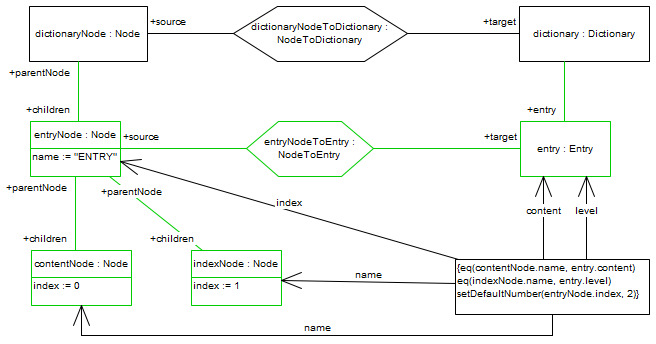
\includegraphics[width=1.1\textwidth]{ea_ForAllEntryRule}
  \caption{\texttt{ForAllEntryRule}}
  \label{ea:ForAllEntry_Complete}
\end{center}
\end{figure}

\subsubsection{AuthorRule} % ---------------------------------

\item[$\blacktriangleright$] Double-click the anchor in the top left of the diagram to return to \texttt{NodeToDictionaryRule}. We want to create a rule to
handle authors next. We can begin our rule by deriving from \texttt{DictionaryNode}, \texttt{dictionary}, and \texttt{shelf}, but we'll need to add a fourth
context element, \texttt{library}, in accordance with the \texttt{Dictionary} metamodel, where each \texttt{author} is connected to its \texttt{dictionary} and
the \texttt{library} instance. Therefore, derive and create \texttt{AuthorRule} as shown in Fig.~\ref{ea:AuthorRule}.

\begin{figure}[h]
  \hspace{-2cm}
  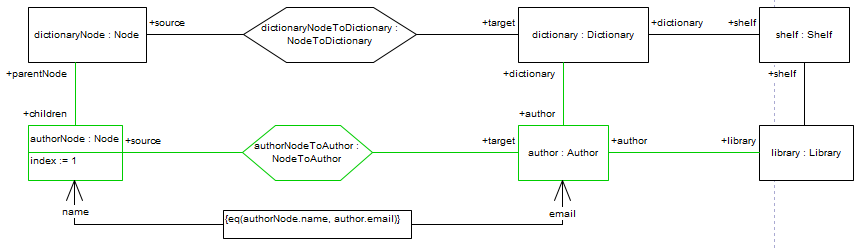
\includegraphics[width=1.3\textwidth]{ea_AuthorRule}
  \caption{\texttt{AuthorRule}}
  \label{ea:AuthorRule}
\end{figure}

\end{itemize}

Handling each \texttt{author} instance, however, can't be realized with a single rule. Right now, we have specified that for every \texttt{authorNode} the
rule finds, an \texttt{author} instance is created. This would be fine if we had unique authors for \emph{every} dictionary \texttt{File}, but if you take look
at both of the french \texttt{numbers} files, you'll notice they both have the same contact information. This means that our \texttt{Dictionary} will have two
identical \texttt{author} instances for one \texttt{library}.

Some users may be okay with this, and not care about redundant information so long as all the correct information is there, while others would prefer a
more concise structure. How can we refine this rule so that it's easy to handle both cases?

eMoflon's visual syntax has a cool \emph{refinement} feature which enables you to adjust specific elements in a rule, without having to redraw a
diagram exactly as before, except for one or two small differences. Our rules to handle either \emph{always} creating an \texttt{author}, or checking for an
existing one first are nearly identical to \texttt{AuthorRule}, save for the binding and reference links on the matched \texttt{authorNode}, so this feature is
exactly what we need.

\begin{itemize}

\item[$\blacktriangleright$] Return to the \texttt{Rules} diagram. Since we're no longer implementing \texttt{AuthorRule} directly, we need to make it
\texttt{abstract}. Select the rule, then hit \texttt{alt + enter} to open its properties dialogue.

\item[$\blacktriangleright$] Switch to the \texttt{Details} tab, and select \texttt{Abstract} from the list of properties (Fig.~\ref{ea:abstractDetails}). 
Affirm and close by pressing \texttt{OK}.

\begin{figure}[htbp]
\begin{center}
  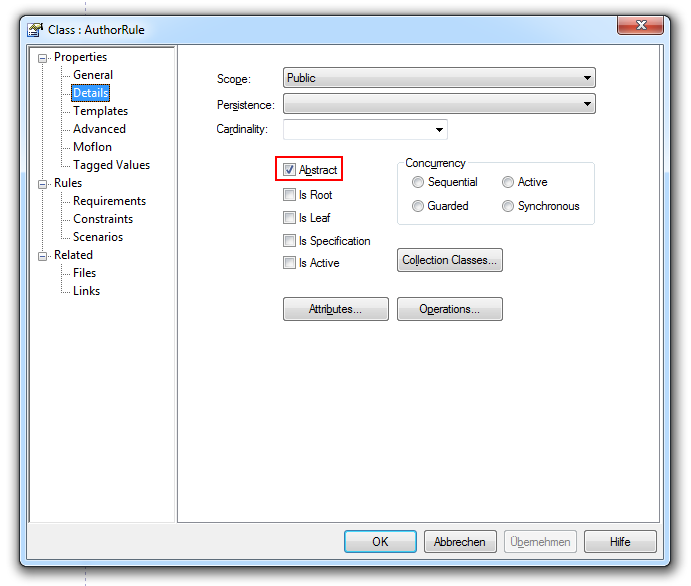
\includegraphics[width=\textwidth]{ea_abstractDetails}
  \caption{Declaring \texttt{AuthorRule} as abstract}
  \label{ea:abstractDetails}
\end{center}
\end{figure}

\end{itemize}

Now we can develop our two rules. The key idea when building refinements is to imagine the rules are being placed directly over the pattern they inherit from,
similar to a transparency sheet. These rules execute \texttt{AuthorRule} exactly, except for whatever modifications you make (which ``cover'' the original
element).

Let's make a rule to handle an already existing author first. Inspecting \texttt{AuthorRule}, we still want the rule to match a new \texttt{authorNode}
and create a link between \texttt{author} and \texttt{dictionary}, but the \texttt{author} element, and the link connecting it to \texttt{library} should
already exist, (i.e., be `black').

\begin{itemize}

\subsubsection{ExistingAuthorRule} % ---------------------------------

\item[$\blacktriangleright$] In \texttt{AuthorRule}'s diagram, select \texttt{authorNode} and \texttt{library}, and press \texttt{Derive}. Enter
\texttt{ExistingAuthorRule} as the rule's name but given that we want to refine the selected elements, not use them as context elements,
be sure to select the \texttt{exact copy} option (Fig.~\ref{ea:deriveRefinement}).

\item[$\blacktriangleright$]

\begin{figure}[htbp]
\begin{center}
  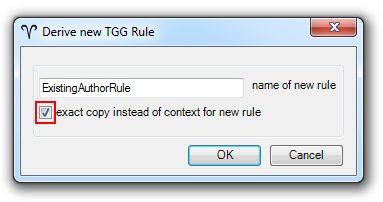
\includegraphics[width=0.6\textwidth]{ea_deriveRefinement}
  \caption{Deriving a refinement rule}
  \label{ea:deriveRefinement}
\end{center}
\end{figure}

\item[$\blacktriangleright$] The rule diagram will open in the editor, with the elements in the same place you copied them from. You can of course rearrange as
you wish, but the overlay idea will  be much easier to visualise if you leave the elements exactly where they are.

\item[$\blacktriangleright$] Complete the rule by changing \texttt{author} and the link to \texttt{library} to \texttt{Check Only} as depicted in
Fig.~\ref{ea:existingAuthorRule}.

\begin{figure}[htbp]
\begin{center}
  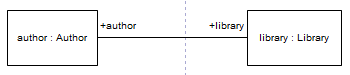
\includegraphics[width=0.7\textwidth]{ea_ExistingAuthorRule}
  \caption{\texttt{ExistingAuthorRule}}
  \label{ea:existingAuthorRule}
\end{center}
\end{figure}

\item[$\blacktriangleright$] \update Include a paragraph about how the rule would have looked w/o refinements (i.e., before the bug). Would be big. (Check
downloads folder; file prepared). Would have exact same semantics as our refinement(s).

\item[$\blacktriangleright$] Mention that, if you want to populate your refinement a little bit more without actually changing anything, EA allows you to drag
and drop all elements from the basis/source rule as links, so they're represented in the diagram. (include screenshot here? it may emphasize the overlay idea..)

\subsubsection{NewAuthorRule} % ---------------------------------

\item[$\blacktriangleright$] Return to \texttt{AuthorRule}. For reasons that will be explained shortly in the next section, derive a copy of \texttt{authorNode}
and \texttt{library} in a rule called \texttt{NewAuthorRule}. Specify it as completely empty, not changing either of the variables for now. It should come to
resemble Fig.~\ref{ea:NewAuthorRule}.\footnote{For presentation purposes, we have reduced the white space between these elements. In your rule they
will be in their original places, far apart.} Since we have defined \texttt{AuthorRule} as abstract, it needs this concrete rule to execute it. 

\vspace{0.5cm}

\begin{figure}[htbp]
\begin{center}
  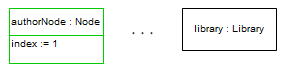
\includegraphics[width=0.6\textwidth]{ea_NewAuthorRule}
  \caption{Completed \texttt{NewAuthorRule}}
  \label{ea:NewAuthorRule}
\end{center}
\end{figure}

\item[$\blacktriangleright$] Of course, we could have left \texttt{AuthorRule} concrete and used just the two rules, but having an explicit abstract rule, with
two concrete implementations of the possibilities, is clearer.

\item[$\blacktriangleright$] Return to the \texttt{Rules} diagram one last time. In order to ensure the new rules will refine \texttt{AuthorRule},
quick-link from each to the root rule, choosing \texttt{Create Refinement Link} from the context menu. Your diagram should now resemble
Fig.~\ref{ea:refinementClasses}.

\item[$\blacktriangleright$] You're nearly done! Make sure everything is saved, and validate your TGG. 

\newpage

\vspace*{2cm}

\begin{figure}[htbp]
\begin{center}
  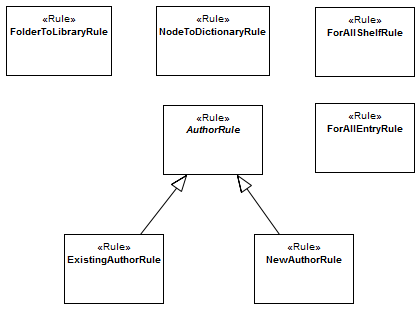
\includegraphics[width=0.7\textwidth]{ea_refinementLinks}
  \caption{Final \texttt{Rules} diagram}
  \label{ea:refinementClasses}
\end{center}
\end{figure}

%If a dialogue appears saying the attempt was
%unsuccessful, you may simply need to update the schema diagram which may not contain the new correspondence types you created on the fly. To do so, open the
%\texttt{DictionaryCodeAdapter} diagram, right-click anywhere in the window and add any missing elements by navigating to ``Insert Existing Element''
%(Fig.~\ref{ea:insertContext}). Selecting the missing correspondence types and the involved classes from the neccessary root package tree
% (Fig.~\ref{ea:insertTree}).

%\vspace{0.5cm}

%\begin{figure}[htbp]
%   \centering
%      \subfloat[Right-click to open the context menu]{
%        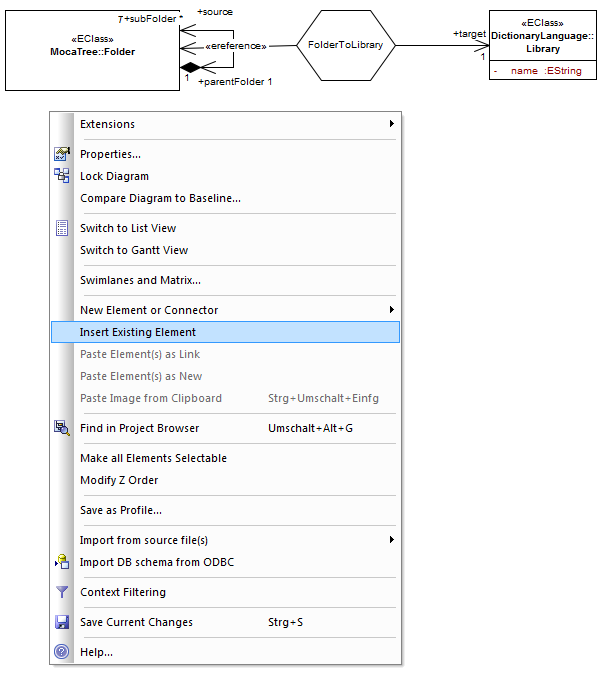
\includegraphics[width=0.7\textwidth]{ea_InsertExistingElements}
%        \label{ea:insertContext}
%      }
%      \\
%      \subfloat[Check your \texttt{TGG}, \texttt{DictionaryLanguage}, and \texttt{MocaTree} packages for elements.]{
%        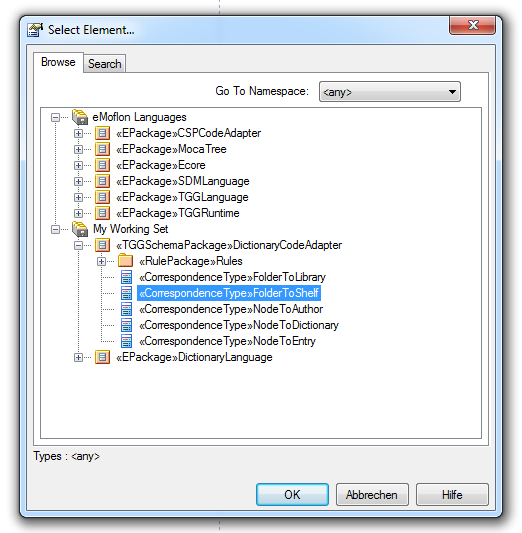
\includegraphics[width=0.7\textwidth]{ea_insertElementTree}
%        \label{ea:insertTree}
%      }
%\end{figure}

% \item[$\blacktriangleright$] Your schema diagram should resemble Fig.~\ref{ea:Schema_Complete} upon exit. Validate the project once again, then switch to the
% Eclipse workspace and refresh the package explorer.

% \newpage

% \vspace*{3cm}

% \begin{figure}[htbp]
%  \hspace{-1.5cm}
%  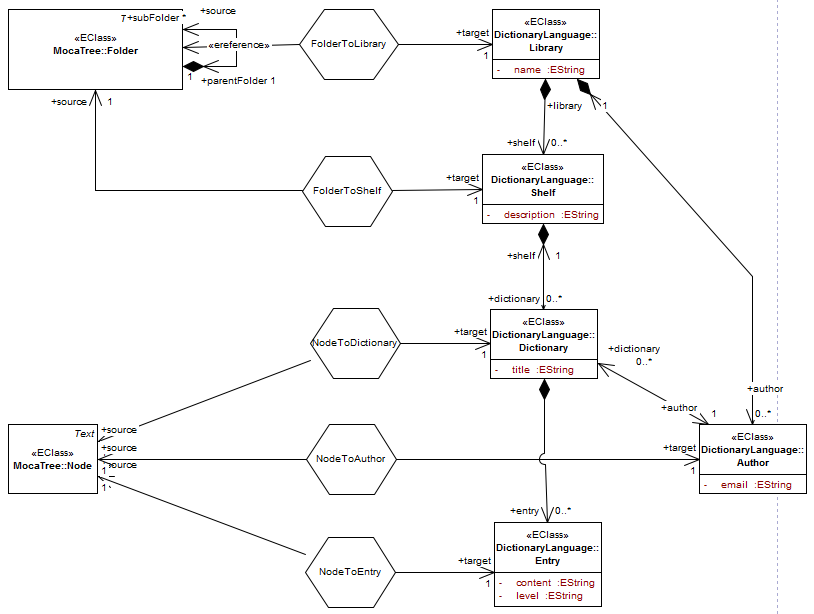
\includegraphics[width=1.3\textwidth]{ea_finalSchema}
%  \caption{The completed TGG Schema}
%  \label{ea:Schema_Complete}
%\end{figure}

\jumpSingle{t2m close}

\end{itemize}
